%
% This file is part of 'isamon'
%
% Copyright (c) 2017, Martin Pumr
% All rights reserved.
%
% Redistribution and use in source and binary forms, with or without
% modification, are permitted provided that the following conditions are met:
%      * Redistributions of source code must retain the above copyright
%        notice, this list of conditions and the following disclaimer.
%      * Redistributions in binary form must reproduce the above copyright
%        notice, this list of conditions and the following disclaimer in the
%        documentation and/or other materials provided with the distribution.
%      * Neither the name of the <organization> nor the
%        names of its contributors may be used to endorse or promote products
%        derived from this software without specific prior written permission.
%
% THIS SOFTWARE IS PROVIDED BY THE COPYRIGHT HOLDERS AND CONTRIBUTORS "AS IS" AND
% ANY EXPRESS OR IMPLIED WARRANTIES, INCLUDING, BUT NOT LIMITED TO, THE IMPLIED
% WARRANTIES OF MERCHANTABILITY AND FITNESS FOR A PARTICULAR PURPOSE ARE
% DISCLAIMED. IN NO EVENT SHALL MARTIN PUMR BE LIABLE FOR ANY
% DIRECT, INDIRECT, INCIDENTAL, SPECIAL, EXEMPLARY, OR CONSEQUENTIAL DAMAGES
% (INCLUDING, BUT NOT LIMITED TO, PROCUREMENT OF SUBSTITUTE GOODS OR SERVICES;
% LOSS OF USE, DATA, OR PROFITS; OR BUSINESS INTERRUPTION) HOWEVER CAUSED AND
% ON ANY THEORY OF LIABILITY, WHETHER IN CONTRACT, STRICT LIABILITY, OR TORT
% (INCLUDING NEGLIGENCE OR OTHERWISE) ARISING IN ANY WAY OUT OF THE USE OF THIS
% SOFTWARE, EVEN IF ADVISED OF THE POSSIBILITY OF SUCH DAMAGE.

%%%%%%%%%%%%%%%%%%%%%%%%%%%%%%%%%%%%%%%%%%%%%%%%%%%%%%%%%%%%%%%%%%%%%
\documentclass[a4paper,11pt,onecolumn,notitlepage]{article}
\usepackage[text={17cm, 24cm},left=2cm,top=3cm]{geometry}
\usepackage[utf8]{inputenc}
\usepackage[czech]{babel}
\usepackage{graphicx}
\usepackage{times}
\usepackage{listings}
\usepackage{color}
\usepackage{hyperref}
\usepackage{lmodern}
\usepackage[T1]{fontenc}
\usepackage{pdfpages}

\lstset{language=C}
\hypersetup{
    colorlinks=true,
    linktoc=all,
    linkcolor=blue,
    citecolor=blue,
    urlcolor=blue,
}

\providecommand{\uv}[1]{\quotedblbase #1\textquotedblleft}

\def \dataDir {data}

%%%%%%%%%%%%%%%%%%%%%%%%%%%%%%%%%%%%%%%%%%%%%%%%%%%%%%%%%%%%%%%%%%%%%
\begin{document}
% ================================================================= %
\begin{center}
    \begin{figure}[hb]
        \centering
        
\includegraphics{\dataDir/FIT.eps}
        \label{fig:FIT}
    \end{figure}
\vspace{\stretch{0.382}}
\LARGE
    Síťové aplikace a správa sítí (ISA)\\
\Huge
    Monitorování sítě\\
\vspace{\stretch{0.618}}
\end{center}

{\Large v~Brně \hfill Martin Pumr (xpumrm00)\\
\today}

\pagenumbering{gobble}
\newpage

\pagenumbering{arabic}

% ================================================================= %
% \section{Obsah}
\tableofcontents
\newpage
% ================================================================= %
\section*{Abstrakt}
\paragraph{} Tato práce popisuje nástroj pro monitorování sítě. V~následujích kapitolách jsou postupně rozepsány metody, pomocí nichž lze zjistit aktivitu stanic v~počítačové síti a provést jejich základní analýzu.
\vspace{7cm}
% ================================================================= %
\section*{Klíčová slova}
Skenování sítě, Skenování portů, port, ethernet, paket, rámec, ping,
OSI/ISO, IEEE 802.3, ARP, ICMP, TCP, UDP,
\newpage
% ================================================================= %

\section{Úvod do problematiky}
\paragraph{} Prvním krokem při skenování sítě, který je třeba učinit je nalezení aktivních stanic. Hledání aktivních stanic se může lišit, podle toho, či je skenovaná síť lokální, nebo naopak vzdálená.
% ----------------------------------------------------------------- %
\subsection{Lokální síť}\label{fig:CHAPTER_LOCAL_NET}
Pokud je skenovaná síť lokální lze v~zásadě použít dva přístupy. Prvním z~nich je zjišťovat aktivní stanice pomocí \textbf{ARP} protokolu, tím druhý je použití \textbf{ICMP} protokolu. Použití \textbf{ICMP} bude popsáno v~kapitole pro skenování vzdálené sítě \ref{fig:CHAPTER_FOREIGN_NET}.

\paragraph{} \textbf{ARP} protokol je definován ve standardu \textbf{RFC 0826} \cite{RFC0826}. Jedná se o~protokol, který operuje dle síťového modelu \textbf{OSI/ISO} \cite{MatousekPetr2014Saaj} na L2 vrstvě. Pro svoji činnost využívá \textbf{ethernet} L1 protokol \textbf{IEEE 802.3} \cite{RFC1042}.

\paragraph{} Základní myšlenka skenování počívá ve vytvoření \textbf{ARP rámce}, obsahující Ethernetovou a ARP hlavičku. Před odesláním je tento paket naplněn příslučnými daty.
\begin{lstlisting}[frame=single,caption={Struktura paketu pro ARP dotaz},captionpos=b]
struct arp_request_t {
    /// Ethernet part       //  Offset
    uint8_t dst_mac[6];     //  0 -  5
    uint8_t src_mac[6];     //  6 - 11
    uint8_t type[2];        // 12 - 13
    /// Arp Part
    uint16_t htype;         // 14 - 15
    uint16_t ptype;         // 16 - 17
    uint8_t hlen;           // 18 - 18
    uint8_t plen;           // 19 - 19
    uint16_t opcode;        // 20 - 21
    uint8_t sender_mac[6];  // 22 - 27
    uint8_t sender_ip[4];   // 28 - 31
    uint8_t target_mac[6];  // 32 - 37
    uint8_t target_ip[4];   // 38 - 41
};
\end{lstlisting}\label{fig:ARP_PACKET}

\paragraph{} Za zmínku stojí hodnoty, které jsou přiřazeny do pole \emph{dst\_mac} a \emph{target\_mac}. Do \emph{dst\_mac} bude dle vložena hodnota \emph{FF:FF:FF:FF:FF:FF}, neboť MAC adresa cíle není v době odesílání známá (je tedy vložena adresa broadcastu). Pole \emph{target\_mac} bude v~žádosti ignorováno a dle \textbf{RFC 5227} \cite{RFC5227} by mělo být nastaveno na hodnotu \emph{00:00:00:00:00:00}.

\paragraph{} Při zachycení ARP paketu si cílová stanice zkontroluje pole \emph{target\_ip}. Pokud je její IP adresa stejná, jako IP adresa v~tomto poli, odešle zpět ARP odpověď, ve které informuje o~své MAC adrese.
% ----------------------------------------------------------------- %
\subsection{Vzdálená síť}\label{fig:CHAPTER_FOREIGN_NET}
\paragraph{} Aktivní skenování, či pasivní poslech, lokální sítě pomocí ARP je spolehlivá technika. Bohužel ji není možné použít pro skenování vzdálených sítí. Jednou z~metod použitelných pro skenování vzdálenách sítí, je využítí protokolu \textbf{ICMP} definovaného v~\textbf{RFC 0777} \cite{RFC0777}. ICMP je protokol operují dle OSI/ISO na L3 vrstvě. Pro svou činnost využívá IP protokol, který operuje taktéž na L3 vrstvě.

\paragraph{} Myšlenka skenování pomocí ICMP protokolu je velmi jednoduchá. Klient odešle ICMP žádost typu \textbf{ECHO}. Pokud je vzdálená stanice aktivní, odpoví ICMP \textbf{ECHO REPLY}. Nevýhodou této techniky je fakt, že ICMP protokol může být blokován síťovými prvky. Rovněž může být limitován maximální počet ICMP zpráv za jednotku času. Pro spolehlivost této metody je nutné, aby takto skenovaná stanice dodržovala standart \textbf{RFC 1122} \cite{RFC1122} (tedy odpovídala na ICMP žádosti a neblokovala je). Za zmínku stojí fakt, že tento mechanismus je používán standartním programem \emph{ping}.

\begin{lstlisting}[frame=single,caption={Struktura výsledného ICMP dotazu},captionpos=b]
#include <netinet/ip.h>         // struct iphdr
#include <netinet/ip_icmp.h>    // struct icmphdr, ICMP_ECHO
...
struct icmp_echo_t {
    /// IP part
    struct iphdr iph;
    /// ICMP part
    struct icmphdr iph;
};
\end{lstlisting}\label{fig:ICMP_ECHO_PACKET}

\subsection{Hledání otevřených portů}
\paragraph{} Hledání otevřených portů je činnost, pomocí které lze zjistit, na~jakých portech lze s~cílovou stanicí komunikovat. Pokud stanice reaguje na pokusy o~navázání spojení, je daný port takzvaně otevřený. V~opačném případě jej lze vyhodnotit jako uzavřený. Přenost skenování lze zvýšit tím, že je na port poslán konkrétní řetězec bajtů. Tento typ skenování předpokládá, že na portu XY, běží síťová služba, která na takto zaslaný řetězec reaguje. Nejčastěji je tento postup používám pro takzvané \textbf{well-known} porty \cite{WIKI_wellKnownPorts}. Tuto metu používá například program \emph{nmap} \cite{DOC_man_NMAP}. Nutno podotknout, že skenování portů je v~některých zemích považováno za ilegální.

% ----------------------------------------------------------------- %
\subsection{TCP porty}\label{fig:CHAPTER_TCP}
\paragraph{} \textbf{TCP} protokol operuje dle modelu \textbf{OSI/ISO} na síťové vrstvě L4. Jeho hlavním úkole je garantovat spolehlivý přenos dat. Pro svoji činnost využívá \textbf{TCP segmenty} \cite{WIKI_TCP}, skrze které data přenáší. Jelikož TCP garantuje spolehlivý přenos, lze díky tomu považovat skenování otevřených portů také za přesné.

\paragraph{} Existuje několik metod, pomocí nichž lze zjistit otevřené TCP porty. Nejjednodušší metodou je prosté volání funkce \emph{connect()}, která je dostupná v~operačním systému. Pokud je volání \emph{connect()} úspěšné, je port otevřený. V~opačném případě je uzavřený. Tato metoda je však velmi \uv{hlučná} a není zcela pod kontrolou. Další známou metodou je skenování pomocí \textbf{TCP SYN} paketů. Tato metoda spočívá v~odeslání TCP paketu s~nastaveným příznakem SYN. Pokud je na skenované stanici port otevřený, stanice ihned odešle \textbf{SYN+ACK} paket. Následně skener ukončí navazované TCP spojení odesláním \textbf{TCP RST} paketu. Oproti skenovní pomocí \emph{connect()}, vykazuje tato metoda nižší počet odeslaných paketů a vyšší rychlost skenování.

\paragraph{} Pro zajímavost je zde uvedeno několik dalších technik, které lze použít pro TCP skenování \textbf{X-Mass}, \textbf{Null-scan}, \textbf{FIN scan} \cite{WIKI_portScanningTechiques}.
% ----------------------------------------------------------------- %
\subsection{UDP porty}\label{fig:CHAPTER_UDP}
\paragraph{} \textbf{UDP} \cite{WIKI_UDP} je protokol operující na L4 vrstvě. Jedná se o~nespolelehlivý, nepotvrzovaný přenos dat. Pro svoji činnost využívá \textbf{UDP datagramy}, pomocí nichž, jsou data přenášena. Jelikož je UDP spojení nepotvrzované, skenování portů zde probíhá zcela odlišným způsobem.

\paragraph{} Jediné co při skenování UDP portů lze s~jistotou říci je, že UDP port je zavřený. Před odesláním žádosti na port předpokládáme, že je otevřený. Pokud do určitého časového intervalu přijde ICMP zpráva typu \textbf{ICMP\_UNREACH} s~kódem \textbf{ICMP\_UNREACH\_PORT}, lze vyhodnotit port jako uzavřený \cite{RFC1122}. V~opačném případě je port otevřený, či filtrovaný (ICMP odpověď zablokoval síťový prvek).
\begin{lstlisting}[frame=single,caption={Struktura příchozího ICMP UNREACH paketu},captionpos=b]
#include <netinet/ip.h>         // struct iphdr
#include <netinet/ip_icmp.h>    // struct icmphdr
                                // ICMP_UNREACH, ICMP_UNREACH_PORT
#include <netinet/udp.h>        // struct udphdr
...
struct icmp_unreach_t {
    struct iphdr iph_res;
    struct icmphdr icmph_unreachResp;
    struct iphdr iph_req;
    struct udphdr udph_req;
    uint8_t * data;
};
\end{lstlisting}\label{fig:ICMP_UNREACH_PORT}
\paragraph{} Výše je ukázka příchozí ICMP odpovědi. v~proměnné \emph{icmph\_unreachResp} je umístěna zpráva ICMP\_UNREACH s~kódem ICMP\_UNREACH\_PORT. Následující tři proměnné obsahují původní zprávu, která byla odeslána na UDP port. Je zde umístěna kopie odesílané IP hlavičky a kopie UDP hlavičky. Proměnná \emph{data} je ukazatelem na data, která byla odeslána v~UDP žádosti. Dle \textbf{RFC 1122} \cite{RFC1122} by zde mělo být alespoň prvních 8 bajtů UDP dat.
% ================================================================= %
\newpage
\section{Logický návrh programu}
\paragraph{} Aplikace \emph{Isamon} byla navržena objektově. \emph{Objektový návrh} umožňuje zachovat modularitu a stejně tak znovupoužitelnost kódu při budoucích změnách.
\begin{figure}[h]
    \centering
    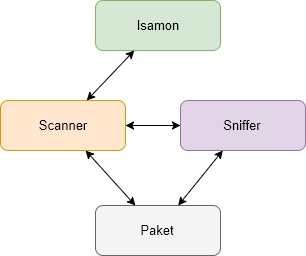
\includegraphics[width=\textwidth,height=60mm,keepaspectratio]{\dataDir/isamon_diagram.png}
    \caption{Objektové schéma aplikace Isamon\label{fig:ISAMON_DIAGRAM}}
\end{figure}
% ----------------------------------------------------------------- %
\subsection{Objekt Isamon}\label{fig:Isamon}
\paragraph{} Hlavní objekt nese jméno výsledné aplikace, \emph{Isamon}. Po spuštění progrmau je zavolán tento objekt. Nejprve provede inicializace (zpracování a ověření argumentů, načtení síťových rozhraní, \dots) a následně zavolá objekt \emph{Skener} \ref{fig:Skener}.
% ----------------------------------------------------------------- %
\subsection{Objekt Skener}\label{fig:Skener}
\paragraph{} Tento objekt se stará o~samotné skenování sítě. Dle nastavení, které mu předal nadřazený objekt \emph{Isamon} \ref{fig:Isamon}, iterativně prochází jednotlivá síťová zařízení a na každém z~nich spustí skenování. V~první fázi zjistí, které IP adresy ze zadaného pásma jsou aktivní. Dále pro všechny aktivní stanice spouští skenování portů.
% ----------------------------------------------------------------- %
\subsection{Objekt Sniffer}\label{fig:Sniffer}
\paragraph{} Objekt \emph{Sniffer} běží paralelně s~objektem \emph{Skener} \ref{fig:Skener}. Úkolem tohoto objektu je příjmat a zpracovávat pakety. Objekt definuje metody, které na samostatných vláknech zpracovávají požadavky, které přišly jako odpovědi na dotazy Skeneru. Zachycené záznamy průběžně předává objektu \emph{Skener} \ref{fig:Skener}.
% ----------------------------------------------------------------- %
\subsection{Objekt Paket}
\paragraph{} Objekt \emph{Paket} byl vytvořen pro lepší práci s~příchozími a odchozími pakety. Definuje datové typy pro jednotlivé pakety v~závislosti na jejich typu (ARP, IP, ICMP, TCP, UDP) a obsahuje metody pro jejich vytváření a zpracování. Objekt paket je aktivně využíván objekty \emph{Skener} \ref{fig:Skener} a \emph{Sniffer} \ref{fig:Sniffer}.

\newpage
% ================================================================= %
\section{Implementační detaily}
\paragraph{} Aplikace byla implementována pomocí jazyka \textbf{C++}. Důvodem byl již zmíněný objektově orientovaný návrh. Odesílání či příjmání paketů je nelbokující a je realizováno pomocí standartních funkcí \emph{sendto()} a \emph{recvfrom()}.

\paragraph{} Omezeních vstupních parametrů je následující. Isamon je schopen skenovat síť v rozasahu \emph{1.0.0.0~239.255.255.255}. Je jím tedy možné oskenovat adresy tří A~D. Adresy třídy E jsou experimentální. Ismaon nezahrnuje třídu E z důvodu implementace TCP/IP stacku v některých operačních systémech, kde je práce s adresami třídy E nedefinována. Omezení pro maximální hodnotu síťové masky se řídí \textbf{RFC 3021} \ref{RFC3021}. Tento dokument říká, že je možné použít masku \emph{31} pro adresování \textbf{Point-to-Point} linek.
% ----------------------------------------------------------------- %
\subsection{ARP a ICMP}
\paragraph{} Jak již bylo zmíněno, prvním krokem je nalezení aktivních stanic. Skenování iniciuje objet \emph{Skenner}, který nejprve vytvoří dva objekty \emph{Sniffer} a následně zavolá jejich metody \emph{ArpStartCapture()} a \emph{IcmpEchoStartCapture()}. Poté postupně začne rozesílat žádosti na jednotlivé stanice. Žádosti jsou vytvářeny objektem \emph{Paket}, konkrétně jeho metodami \emph{forgeArpRequest()} a \emph{forgeIcmpEcho()}. Po odeslání posledních paketů je Sniffer zastaven a výsledek jeho činnosti navrácen Skeneru, který data zpracuje a případně vypíše na standartní výstup.
\begin{figure}[h]
    \centering
    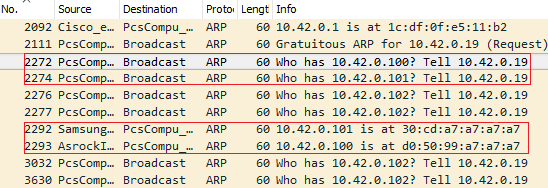
\includegraphics[width=\textwidth,height=\textheight,keepaspectratio]{\dataDir/arp.png}
    \caption{ARP žádost a následná ARP odpověď\label{fig:SHARK_ARP}}
\end{figure}
\begin{figure}[h]
    \centering
    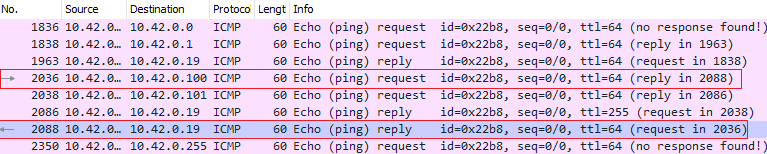
\includegraphics[width=\textwidth,height=\textheight,keepaspectratio]{\dataDir/icmp_echo.png}
    \caption{ICMP ECHO a následné ICMP ECHO REPLAY\label{fig:SHARK_ICMP_ECHO}}
\end{figure}
\paragraph{} Obrázky \ref{fig:SHARK_ARP} a \ref{fig:SHARK_ICMP_ECHO} zobrazují Výše popsanou činnost v~praxi.
% ----------------------------------------------------------------- %
\subsection{Skenování TCP portů}
\paragraph{} Pro skenování TCP portů byly použity dvě metody. První z~nich je základní metoda používající standartní funkci \emph{connect()}. Bohužel se takto prováděné iterativní skenování příliš neosvědčilo a nepomohla ani jeho paralelizace. Proto byla metoda vyřazena (zdrojové kódy byly zachovány) a nahrazena metodou používající TCP SYN pakety \ref{fig:CHAPTER_TCP}. Pokud je nastaven příslušný argument, Skenner nejprve vytvoří objekt Sniffer a následně zavolá jeho metodu \emph{StartTcpCapture()}. Poté začne iterativně odesílat TCP SYN žádosti na jednotlivé porty. Tyto žádosti jsou opět vytvářeny pomocí objektu Paket, \emph{forgeTcpSyn()}. Po vypršení času Skener postupně začne odesílat pakety typu TCP RST (\emph{forgeTcpRst()}), aby došlo k~ukončení navázaného TCP spojení. Nutno podotknout, že SYN a RST pakety jsou odesílány postupně v~dávkách. Důvodem je prevence DOS útoku zvaného SYN FLOOD \cite{WIKI_SYNFlood}. Po skončení skenování je Sniffer pozastaven, a jeho výsledky předány skeneru. Aby nedocházelo k~přeslechům a Sniffer příjmal TCP pakety pouze od stanice, která je aktuálně skenována, je mu její IP adresa předána při inicializaci. Pakety, které nepocházejí od této stanice jsou zahozeny. Na obrázku \ref{fig:TCP} je zobrazena probíhající komunikace. Dotaz na port 22 byl úspěšný.
\begin{center}
\begin{figure}[h]
    \centering
    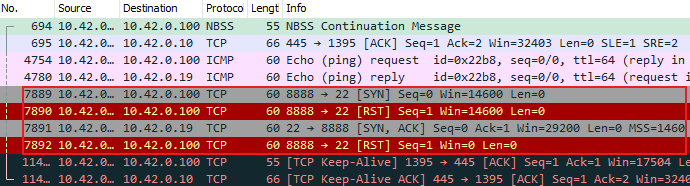
\includegraphics[width=\textwidth,height=\textheight,keepaspectratio]{\dataDir/tcp_open_22.png}
    \caption{TCP SYN žádost a následná TCP ACK odpověď\label{fig:TCP}}
\end{figure}
\end{center}
% ----------------------------------------------------------------- %
\subsection{Skenování UDP portů}
\paragraph{} Skenování UDP portů je opět realizováno pomocí dvou vláken. Skener nejprve Inicializuje objekt Sniffer a volá jeho metodu \emph{IcmpUdpStartCapture()}. Poté poté iterativně odesílá žádosti na jednotlivé UDP porty. Pokud do zadaného časového intervalu přijde zpět odpověd ICMP UNREACH \ref{fig:CHAPTER_UDP}. Je port považován za zavřený. V~opačném případě Isamon vyhodnotí port jako otevřený a vypíše ho na standartní výstup. Na níže uvedeném obrázku \ref{fig:ICMP_UNREACH} je zobrazen UDP dotaz a následná ICMP UNREACH odpovědi, port je tedy s~jistotou zavřený.
\begin{figure}[h]
    \centering
    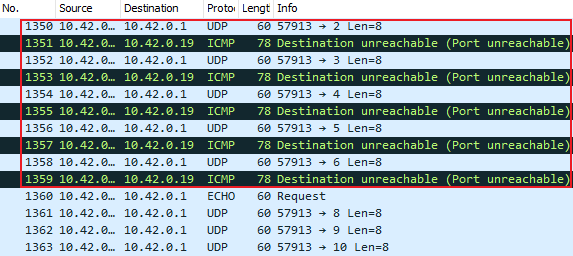
\includegraphics[width=\textwidth,height=\textheight,keepaspectratio]{\dataDir/icmp_unreach.png}
    \caption{Zaslání UDP dotazu a následné přijetí ICMP UNREACH zprávy\label{fig:ICMP_UNREACH}}
\end{figure}

% ================================================================= %
\newpage
\section{Adresářová a Souborová struktura projektu}
\begin{itemize}
\item \textbf{src/} Zde jsou umístěny zdrojové kódy aplikace Isamon
\item \textbf{doc/} Zde jsou umístěny zdrojové texty dokumentace
\item \textbf{doc/data/} Zde jsou umístěny data (obrázky, \dots) pro dokumentaci
\item \textbf{provision-shell/} Umístění konfiguračních skriptů pro Vagrand
\item \textbf{license} Licenční podmínky pro zdrojové texty
\item \textbf{Makefile} Globální Makefile (postupně volá Makefile v~jednotlivých podadresářích)
\item \textbf{README} Soubor v~značkovacím jazyku Markdown, který popisuje jak aplikaci použít
\item \textbf{test.sh} Skript provádějící základní testování aplikace
\item \textbf{Vagrantfile} Upravený konfigurační soubor pro Vagrand
\end{itemize}

\newpage
% ================================================================= %

\bibliographystyle{csplain}
\bibliography{manual}

\newpage
% ================================================================= %
\end{document}
